\documentclass[12pt,a4paper]{report}
\usepackage[T1]{fontenc}
\usepackage[utf8]{inputenc}
\usepackage{charter}
\usepackage{ngerman}
\usepackage{amsmath}
\usepackage[left=2cm,right=2cm,top=2cm,bottom=2cm]{geometry}
\usepackage{graphicx}
\renewcommand\thesection{\arabic{section}.} 

\begin{document}
\title{Abituraufgaben 2023 Vektoren}
\author{Moritz \and Julina \and Ben \and Tanel}
\date{\today}
\maketitle

\section{Aufgabe a) (1)}
\begin{align*}
	B_1(10/-5/30)
\end{align*}
\section{Aufgabe a) (2)}
Die von den zwei Punkten eingegrenzte Fläche hat vier Ecken, und vier Seiten, von denen nur zwei parallel sind:
\begin{align*}
	\overrightarrow{B_2B_3} &= \begin{pmatrix}\frac{\sqrt{75}}{3} - 10 \\ 0 \\ 0\end{pmatrix} \\
	\overrightarrow{A_2A_3} &= \begin{pmatrix}\frac{\sqrt{75}}{3} - 50 \\ 0 \\ 0\end{pmatrix} \\
	(\frac{\sqrt{75}}{3}-10) \cdot x &= \frac{\sqrt{75}}{3} - 50 \\
	\Leftrightarrow x &= \frac{8\cdot\sqrt{3}+59}{11}
\end{align*}
\\
Durch diese Rechnung ergibt sich, dass die zwei Richtungsvektoren Vielfache voneinander sind, also parallel liegen.

\paragraph{Volumen des Körpers K}:
\begin{align*}
	A_G &= \frac{1}{2} \cdot (a+c) \cdot h \\
	&= \frac{1}{2} \cdot (|\overrightarrow{A_2A_3}| + |\overrightarrow{B_2B_3}|) \cdot |\overrightarrow{A_3B_3}| \\
	&\approx \frac{1}{2} \cdot (47.11 + 7.11) \cdot 30 \\
	&\approx 813.3 \\
	V_K &= A_G \cdot |\overrightarrow{A_3A_4}| \\
	&= A_G \cdot 10 \\
	&= 8133VE
\end{align*}

\section{Aufgabe b) (1)}
\begin{align*}
	\overrightarrow{A_2B_2} &= \begin{pmatrix}
 		10\\5\\30	
	\end{pmatrix} + r \cdot \begin{pmatrix}
		40 \\0 \\-30
	\end{pmatrix} \\
	\overrightarrow{A_2B_2} &= \begin{pmatrix}
		50-a \\5\\0.75\cdot a
	\end{pmatrix} \\
	\Rightarrow r &\leq 1
\end{align*}
\section{Aufgabe b) (2)}
\begin{align*}
	\overrightarrow{n} &= \begin{pmatrix}
		0\\0\\10
	\end{pmatrix} \\
	g : \overrightarrow{x} &= \begin{pmatrix}
		41\\-5\\9
	\end{pmatrix} + r \cdot \begin{pmatrix}
		0\\0\\10
	\end{pmatrix} \\
	g &= \overrightarrow{A_2B_2} \\
	\overrightarrow{x} &= \begin{pmatrix}
		38 \\ 5 \\ 9
	\end{pmatrix} + 0 \cdot \begin{pmatrix}
		0 \\ -10 \\ 0
	\end{pmatrix} + 3 \cdot \begin{pmatrix}
		1 \\ 0 \\0
	\end{pmatrix} \\
	&= \begin{pmatrix}
		41 \\ 5 \\ 9
	\end{pmatrix} \\
	S_1: \overrightarrow x &= \begin{pmatrix}
		41\\5 \\9
	\end{pmatrix} + a  \cdot \begin{pmatrix}
		0\\0\\10
	\end{pmatrix} \\
	S_1 &= g \\
	\xrightarrow{CAS} r &= \frac{31}{40} \land a = \frac{-9}{40} \\
	\text{r einsetzen} \\
	SP(41/5/\frac{27}{4}) \\
	|\begin{pmatrix}41\\5\\9\end{pmatrix}| &= \frac{9}{4}
\end{align*}

\section{Aufgabe c) (1)}

\begin{align*}
	|\overrightarrow{A_4A_3}| &= 	\sqrt{0^2 + 10^2 + 0^2} \\
	&= 10LE \\
	|M_{A_3A_4}| &= \begin{pmatrix}
		\frac{\sqrt{75}}{3} \\ 0 \\ 0
	\end{pmatrix}\\
	|\overrightarrow{M_{A_3A_4}A_3}| &= 5LE \\
	|A_3P| &= 10LE \\
	10^2 &= x^2 + 5^2 \\
	x &= 5 \cdot \sqrt{3} \\
	P&\begin{pmatrix}
		M_{A_3A_4}_1 - x \\ 0 \\ 0
	\end{pmatrix} \\
	P&\begin{pmatrix}
		\frac{\sqrt{75}}{3} - 5 \cdot \sqrt{3} \\ 0 \\ 0
	\end{pmatrix} \\
	P&\begin{pmatrix}
		\frac{-10\cdot \sqrt{3}}{3} \\ 0 \\ 0
	\end{pmatrix}
\end{align*}

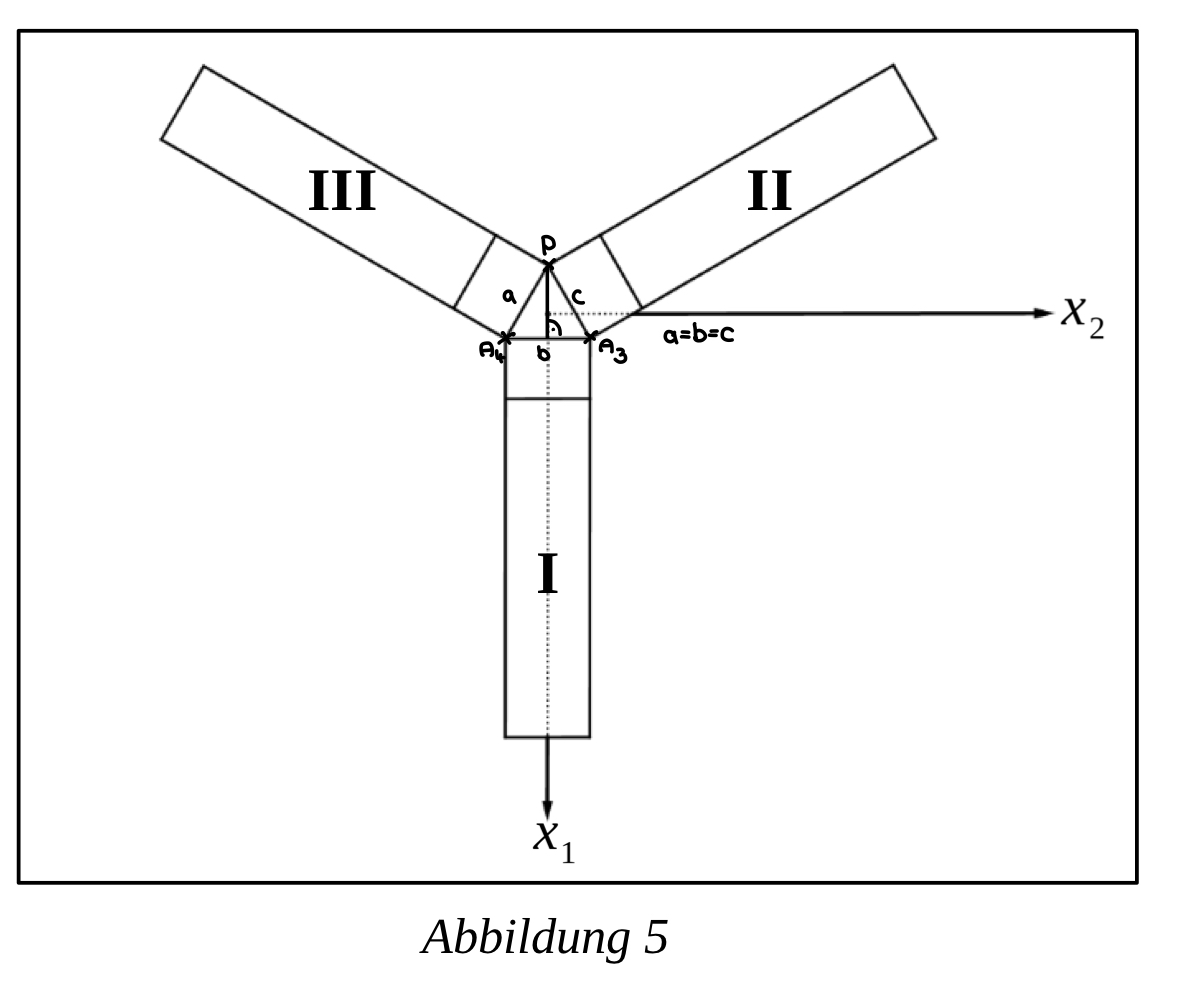
\includegraphics[width=0.5\textwidth]{JPEG-Bild-4AB4-BB3E-2D-0.JPEG}


\section{Aufgabe c) (2)}
\begin{align*}
	|\overrightarrow{A_4O}| &= \sqrt{(\frac{\sqrt{75}}{3})^2 +(-5)^2 + 0^2} \\
	&= \frac{10 \cdot \sqrt{3}}{3}
\end{align*}

\section{Aufgabe d) (1)}
\begin{align*}
	SV &= \overrightarrow{A_1} &= \begin{pmatrix}
		50\\-5\\0
	\end{pmatrix}\\
	RV_1 &= \overrightarrow{A_1A_2} &= \begin{pmatrix}
		50 - 50\\ 5+5 \\ 0-0
	\end{pmatrix}\\ \\
	&&= \begin{pmatrix}
		0 \\10 \\ 0
	\end{pmatrix} \\
	RV_2 &= \overrightarrow{A_1B_1} &= \begin{pmatrix}
		10 - 50 \\ -5 - (-5)\\ 30 -0 
	\end{pmatrix}\\
	&&= \begin{pmatrix}
		-40 \\ 0 \\ 30
	\end{pmatrix} \\
	F: \overrightarrow{x} &= \begin{pmatrix}
		50\\-5\\0
	\end{pmatrix} + r \cdot \begin{pmatrix}
		0 \\ 10 \\0
	\end{pmatrix} + s \cdot \begin{pmatrix}
 		-40 \\ 0 \\ 30	
	\end{pmatrix} \\
	\overrightarrow{n} &= \begin{pmatrix}
		300 \\ 0 \\ 400
	\end{pmatrix} \\
	300 \cdot x_1 + 0 \cdot x_2 + 400 \cdot x_3 &= d \\
	300 \cdot 50 + 400 \cdot 0 &= d \\
	15.000 &= d \\
	F&: 3x_1 + 4x_3 = 150 \\
\end{align*}

\section{Aufgabe d) (2)}
\begin{align*}
	g: \overrightarrow{x} &= \begin{pmatrix}
		0\\0\\35
	\end{pmatrix} + z \cdot \begin{pmatrix}
		6 \\ 0 \\ -2
	\end{pmatrix} \\
	 g &= F \\
	 3 \cdot (0+6z) +4 \cdot 35-2z &= 150 \\
	 \Rightarrow z &= 1 \\
	 S&(6/0/33)
\end{align*}

Der Schatten der Spitze liegt nicht innerhalb der Fläche, da $_3=33 > 30 (\text{Ebene})$

\end{document}